\PassOptionsToPackage{table,xcdraw}{xcolor}

%% For double-blind review submission, w/o CCS and ACM Reference (max submission space)
\documentclass[acmsmall,nonacm]{acmart} 
\pagestyle{plain} % removes running headers

\bibliographystyle{ACM-Reference-Format}
%\citestyle{acmauthoryear}   %% For author/year citations

\usepackage{url}
\usepackage{amsmath}
\usepackage{amsfonts}
\usepackage{amssymb}
\usepackage{listings}
\usepackage{color}
\usepackage{graphicx}

%% https://github.com/nickgian/thesis/blob/master/lstcoq.sty
\usepackage{color}

\definecolor{ltblue}{rgb}{0,0.4,0.4}
\definecolor{dkblue}{rgb}{0,0.1,0.6}
\definecolor{dkgreen}{rgb}{0,0.35,0}
\definecolor{dkviolet}{rgb}{0.3,0,0.5}
\definecolor{dkred}{rgb}{0.5,0,0}

% lstlisting coq style (inspired from a file of Assia Mahboubi)
%
\lstdefinelanguage{Coq}{ 
%
% Anything betweeen $ becomes LaTeX math mode
mathescape=true,
%
% Comments may or not include Latex commands
texcl=false, 
%
% Vernacular commands
morekeywords=[1]{Section, Module, End, Require, Import, Export,
  Variable, Variables, Parameter, Parameters, Axiom, Hypothesis,
  Hypotheses, Notation, Local, Tactic, Reserved, Scope, Open, Close,
  Bind, Delimit, Definition, Let, Ltac, Fixpoint, CoFixpoint, Add,
  Morphism, Relation, Implicit, Arguments, Unset, Contextual,
  Strict, Prenex, Implicits, Inductive, CoInductive, Record,
  Structure, Canonical, Coercion, Context, Class, Global, Instance,
  Program, Infix, Theorem, Lemma, Corollary, Proposition, Fact,
  Remark, Example, Proof, Goal, Save, Qed, Defined, Hint, Resolve,
  Rewrite, View, Search, Show, Print, Printing, All, Eval, Check,
  Projections, inside, outside, Def},
%
% Gallina
morekeywords=[2]{forall, exists, exists2, fun, fix, cofix, struct,
  match, with, end, as, in, return, let, if, is, then, else, for, of,
  nosimpl, when},
%
% Sorts
morekeywords=[3]{Type, Prop, Set, true, false, option},
%
% Various tactics, some are std Coq subsumed by ssr, for the manual purpose
morekeywords=[4]{pose, set, move, case, elim, apply, clear, hnf,
  intro, intros, generalize, rename, pattern, after, destruct,
  induction, using, refine, inversion, injection, rewrite, setoid_rewrite, congr,
  unlock, compute, ring, field, fourier, replace, setoid_replace, fold, unfold,
  change, cutrewrite, simpl, have, suff, wlog, suffices, without,
  loss, nat_norm, assert, cut, trivial, revert, bool_congr, nat_congr,
  symmetry, transitivity, auto, split, left, right, autorewrite},
%
% Terminators
morekeywords=[5]{by, done, exact, reflexivity, tauto, romega, omega,
  assumption, solve, contradiction, discriminate},
%
% Control
morekeywords=[6]{do, last, first, try, idtac, repeat},
%
% Comments delimiters, we do turn this off for the manual
morecomment=[s]{(*}{*)},
%
% Spaces are not displayed as a special character
showstringspaces=false,
%
% String delimiters
morestring=[b]",
morestring=[d]’,
%
% Size of tabulations
tabsize=3,
%
% Enables ASCII chars 128 to 255
extendedchars=false,
%
% Case sensitivity
sensitive=true,
%
% Automatic breaking of long lines
breaklines=false,
%
% Default style fors listings
basicstyle=\small,
%
% Position of captions is bottom
captionpos=b,
%
% flexible columns
basewidth={2em, 0.5em},
columns=flexible,
%
% Style for (listings') identifiers
identifierstyle={\ttfamily\color{black}},
% Style for declaration keywords
keywordstyle=[1]{\ttfamily\bfseries\color{dkviolet}},
% Style for gallina keywords
keywordstyle=[2]{\ttfamily\bfseries\color{dkgreen}},
% Style for sorts keywords
keywordstyle=[3]{\ttfamily\bfseries\color{ltblue}},
% Style for tactics keywords
keywordstyle=[4]{\ttfamily\color{dkblue}},
% Style for terminators keywords
keywordstyle=[5]{\ttfamily\color{dkred}},
%Style for iterators
%keywordstyle=[6]{\ttfamily\color{dkpink}},
% Style for strings
stringstyle=\ttfamily,
% Style for comments
commentstyle={\ttfamily\itshape\color{dkgreen}},
%
%moredelim=**[is][\ttfamily\color{red}]{/&}{&/},
literate=
    {fun}{{\color{dkgreen}{$\lambda\;$}}}1
    {bool}{{$\mathbb{B}$}}1
    {nat}{{$\mathbb{N}$}}1
    {Vforall2}{Vforall2}1 % quick workardoun to avoid partial replacement of 'forall' in identifier
    {nat\_equiv}{nat\_equiv}1 % quick workardoun to avoid partial replacement of 'nat' in identifier
    {forall}{{\color{dkgreen}{$\forall\;$}}}1
    {exists}{{$\exists\;$}}1
    {<-}{{$\leftarrow\;\;$}}1
    {=>}{{$\Rightarrow\;\;$}}1
    {==}{{\texttt{==}\;}}1
    {==>}{{$\Longrightarrow\;\;$}}1
%    {:>}{{\texttt{:>}\;}}1
    {->}{{$\rightarrow\;\;$}}1
    {<-->}{{$\longleftrightarrow\;\;$}}1
    {<->}{{$\leftrightarrow\;\;$}}1
    {<==}{{$\leq\;\;$}}1
    {\#}{{$^\star$}}1 
    {\\o}{{$\circ\;$}}1 
%    {\@}{{$\cdot$}}1 
    {\/\\}{{$\wedge\;$}}1
    {\\\/}{{$\vee\;$}}1
    {++}{{\texttt{++}}}1
    {~}{{\ }}1
    {¬}{{$\lnot$}}1     % this does not work
    {\@\@}{{$@$}}1
    {\\mapsto}{{$\mapsto\;$}}1
    {\\hline}{{\rule{\linewidth}{0.5pt}}}1
%
}[keywords,comments,strings]

\lstnewenvironment{coq}{\lstset{language=Coq}}{}

% pour inliner dans le texte
\def\coqe{\lstinline[language=Coq, basicstyle=\small]}
% pour inliner dans les tableaux / displaymath...
\def\coqes{\lstinline[language=Coq, basicstyle=\scriptsize]}

%%% Local Variables: 
%%% mode: latex
%%% Local IspellDict: british
%%% TeX-master: "main.tex"
%%% End: 
\usepackage{booktabs} 
\usepackage{subcaption}

\newcommand{\N}{\mathbb{N}}

\usepackage{amsmath}
\usepackage{amssymb}
\usepackage{latexsym}
\usepackage{relsize}
\usepackage{xcolor}
\usepackage{color}
\usepackage{mathtools}

%\usepackage{multicol}

\lstset{
  basicstyle=\ttfamily\small,
  frame=tb, % draw a frame at the top and bottom of the code block
  tabsize=4, % tab space width
  showstringspaces=false, % don't mark spaces in strings
  numbers=left, % display line numbers on the left
  commentstyle=\color{green}, % comment color
  keywordstyle=\color{blue}, % keyword color
  stringstyle=\color{red}, % string color
  % identifierstyle=\color{grey},
}

\lstdefinelanguage{diff}{
    morecomment=[f][\color{diffstart}]{@@},
    morecomment=[f][\color{diffincl}]{+},
    morecomment=[f][\color{diffrem}]{-},
  }

\begin{document}

\title{Formally-Verified ASN.1 Protocol C-language Stack}
\subtitle{Work-in-Progress Report}

\author{Nika Pona}
\affiliation{
  \institution{Digamma.ai}
}
\email{npona@digamma.ai}
\author{Vadim Zaliva}
\affiliation{
  \institution{Carnegie Mellon University}
  \department{ECE}
}
\email{vzaliva@cmu.edu}

\begin{abstract}

\end{abstract}

\maketitle

\tableofcontents

\section{Introduction}

\subsection{Background}

The pervasively deployed and widely adopted ASN.1 (``Abstract Syntax
Notation One'') \cite{TODO} joint standard of the International
Telecommunication Union (ITU-T) and the International Organization for
Standardization (ISO/IEC) provides an essential interface description
language for defining data structures for serialized and deserialized
cross-platform data exchange, broadly used in telecommunications,
computer networking, the Internet, and cryptography. ASN.1 is
vitally-relied upon by core aspects of the Internet infrastructure and
Internet applications such as telephony, enterprise computing,
utilities, finance, military, security, digitally-controlled
infrastructure, transportation, medical systems, and commercial cloud
computing.

A simple example of ASN.1 module defining the messages (data
structures) of dummy \textit{Foo} Protocol is shown in
Listing~\ref{lst:asnex}.

\begin{lstlisting}[language=C,label=lst:asnex,
  caption={ASN.1 example}]  
    FooProtocol DEFINITIONS ::= BEGIN
    FooQuestion ::= SEQUENCE {
      someNumber INTEGER,
      question IA5String
    }
    
    FooAnswer ::= SEQUENCE {
      someOtherNumber INTEGER,
      answer BOOLEAN
    }
\end{lstlisting}

A typical ASN.1 stack comprises of a \textit{compiler} which parses
ASN.1 syntax definitions as shown in the Listing~\ref{lst:asnex} and
produces either a source code of a specialized protocol encoder and
decoder for this data or a runtime data for a parametric protocol
encoder and decoder.

However, the ASN.1 standard \cite{TODO} is large and complex:
currently, it comprises twelve sub-standards spanning 862 pages
supplemented by additional pages of corrigenda\cite{TODO}. This opens
a door for many potential software bugs and malicious exploits.
  
\subsection{Motivation}

Proliferating embedded and user computing devices are implementing
vast numbers of essential functions and applications, all of which
exchange data using ASN.1. The resulting interconnected communicating
systems are becoming riskier, less stable, less reliable, and
potentially dangerous. Disruption of the ASN.1 based communications
could threaten the functioning of the critical infrastructure our
society relies upon.


The Computer Vulnerabilities and Exposures (CVE) database
\cite{TODO:7a} lists critical ASN.1-related bugs found each year in
the existing systems, and there have already been noteworthy exposures
\cite{TODO:8} that although not as dire to security as first feared
\cite{TODO:9} clearly spell out a first awareness of the vast risk and
exposure. We analyzed the last 4 years of ASN.1-related issues
reported in Computer Vulnerabilities and Exposures (CVE) database
\cite{TODO:7b}. Among vulnerabilities studied were CVEs for various
software and hardware products and vendors, including \textit{Apple},
\textit{axTLS}, \textit{Botan}, \textit{Bounty Castle},
\textit{librcrypto++}, \textit{libtasn}, \textit{LibTomCrypt},
\textit{Linux Kernel}, \textit{MatrixSSL}, \textit{Mozilla NSS
  (Firefox)}, \textit{Objective Systems}, \textit{OpenSSL},
\textit{PolarSSL}, \textit{RSA BSAFE}, \textit{Samba},
\textit{Samsung}, \textit{Snapdragon}, \textit{strongSwan}, and
\textit{Wireshark}. It was found that 39 out of 52 problems analyzed
were related to memory safety, 6 related to stack and heap bounds
checking, and 3 related to issues caused by applications accepting not
well-formed ASN.1 input. Having proved just six formal properties
would have prevented 49 out of 52 vulnerabilities, that is, more than
90\% of reported vulnerabilities.

\subsection{Our approach}

Systems and methods to date either (a) automatically tested but not
formally verified (b) use verification approach which rely on
automatic extraction from executable specifications (for example
involving network stack synthesis \cite{TODO:31}, optimizing compilers
\cite{TODO:3}, cryptographic libraries \cite{TODO:6}, and
encoder/decoders \cite{TODO:32}), or (c) apply a form of formal
verification which only proves partial correctness properties (partial
verification of NAT stack only proving parts of DPDK are specification
compliant \cite{TODO:33}, partial verification of Linux kernel TCP
implementation with 55\% line coverage and 92\% protocol coverage
\cite{TODO:34}). Consequently, (a) and (c) do not provide sufficient
correctness guarantees, while (c) is often impractical due to poor
performance and compatibility limitations. In contrast, we pursue a
far deeper and comprehensive verification approach to performance and
portability and seek to prove actual industrial-level C-code
implementation.

\section{Preliminary work}

\subsection{Verifying floating-point numbers encoding}

% TODO: summarize @zoick paper, cite it and link to github repository

\subsection{Verifying simple function}

To estimate an effort required to formally verify C code and to
experiment with various verification strategies we decided to try to
verify a small real function from existing ASN.1 compiler. We chose
function \texttt{asn\_strtoimax\_lim} from \texttt{asn1c} compiler.
The function is relatively simple, but at the same time uses many
features of C that make verifying imperative programs
challenging. \emph{XER} decoding functions for \emph{INTEGER},
\emph{OBJECT-IDENTIFIER} and \emph{RELATIVE-OID} types (and hence all
constructed types that use these primitive types) critically depend on
this function.

The only specification provided was the following comment in the
source code. Additional specification details have to be inferred from
the source code and usage examples.

\begin{quote}
 { \it Parse the number in the given string until the given *end position,
 returning the position after the last parsed character back using the
 same (*end) pointer.
 WARNING: This behavior is different from the standard strtol/strtoimax(3). }
\end{quote}

Full source code of the function is included in the Appendix~\ref{sec:stritomax}.

\subsubsection{Bugs}

Despite that fact that this function lineage could be traced back 15
years, and it being a part of mature, well-tested ASN.1 compiler used
many production systems during our formal verification exercise we
found three bugs in current implementation. These bugs were never
reported before and passed all human code reviews, unit, and fuzzying
tests. The following bugs were reported to product developers,
acknowledged and promptly fixed:
  
\paragraph{Negative range bug}

When we go beyond allowed \textit{int} range, a wrong result is given
for some inputs. For example, assuming we are working on a 8-bit
system and the maximum signed integer value is 127, parsing the input
string \texttt{``-1281''} produces the as a result
\emph{ASN\_STRTOX\_OK} with the value -127 instead of expected
\emph{ASN\_STRTOX\_ERROR\_RANGE}. This happens whenever the input
string represents a number smaller than \texttt{MIN\_INT}, due to the
fact that absolute value of \texttt{MIN\_INT} is greater than
\texttt{MAX\_INT}, thus negative number cannot be treated as
$\mathrm{value}\times\mathrm{sign}$ when $\mathrm{value}$ is
represented as \textit{int}. The bug was filed and promptly fixed by
developers:

\paragraph{Memory store bug}

Another bug we discovered was related to potentially overlapping
memory areas pointed by argument pointers. Under some circumstances
the value of the \texttt{end} pointer parameter is treated as a part
of the input data and the resulting error value could be
incorrect. This bug could never occur if the function is always called
with non-overlapping pointer arguments. However this could be viewed
as an implicit pre-condition which should be part of the function's
specification.

\paragraph{Specification Ambiguity}

After addressing the two bugs we discovered we were able to
successfully verify that the function finally corresponds to the
specification we wrote for. However, it was noticed the following
behavior: For input \texttt{``a''} it stores value 0 and returns {\color{green}\texttt{ASN\_STRTOX\_EXTRA\_DATA}} (same behaviour as on input \texttt{``0a''}), which could be unintended by authors. \\

  
\subsubsection{Direct operational semantics proof}
First we formulated functional correctness and proved it using big-step operational semantics of C light, defined in Compcert. In this proof we used a Coq abstraction of C function \texttt{asn\_strtoimax\_lim : addr -> addr -> addr -> option asn\_strtoimax\_lim\_result} as as an intermediate specification in the proof. 

\begin{lstlisting}[language=Coq]
(* Return type *)
Record asn_strtoimax_lim_result :=
 { return_type : asn_strtox_result ;
   value : option int64 ;
   end_pointer : option addr ;
   memory : option mem 
   }.

\end{lstlisting}

This function took addresses as inputs and operated on memory using \texttt{load} and \texttt{store} operations from CompCert's memory model, while calculating the resulting machine integer value. The proof went by induction on the distance between input pointers and the main difficulty apart trying to prove a faulty program (that's when we discovered two bugs) was operational semantics control flow minuities and machine arithmetic proofs. However, only a couple of lemmas about the spec were needed. However, since functional and memory specification were intertangled it was more difficult to read the spec and make sure it was correct. 

\subsubsection{Proof using VST}

Verified Software Toolchain provided solutions to problems we encountered while doing direct opertational semantics proof: it has good automation of control flow, some automation for machine arithmetic and clearly separates functional and memory-related parts of the specification. It also provides a uniform way of stating functional correctness and memory safety. Proofs here are done in Hoare and separation logics, which are proven to be sound with respect to operational semantics. VST has tactics that can solve simple entailments in these logics, however, they were not powerful enough to significantly reduce the proof effort. In fact, with respect to memory specifications, direct operational semantics proof was shorter and more straightforward.

\paragraph{Specification layers} First we have a high-level specification of this function in declarative, relational style. Each constructor corresponds to a return message (state) and stores value the number of iterations of the function (used to store the result).

 \begin{lstlisting}[language=Coq]

(* Relation between input string, value, index an asn_strtox_result_e message *)
  Inductive asn_strtoimax_lim : list byte -> Z -> Z -> asn_strtox_result_e -> Prop :=
  (* Invalid data encountered *)
  | ERROR_INVAL:
      asn_strtoimax_lim nil 0 0 ERROR_INVAL
  (* More data expected (e.g. "+") *)
  | EXPECT_MORE : forall ls c,
      ls = [c]  ->
      is_sign c = true ->
      asn_strtoimax_lim ls 0 1 EXPECT_MORE
 (* Non-digit encountered *)
  | EXTRA_DATA : forall c ls z i,
      asn_strtoimax_lim ls z i OK ->
      is_digit c = false -> 
      asn_strtoimax_lim (ls ++ [c]) z i EXTRA_DATA
   ...    
  \end{lstlisting}

Next level is executable specification \texttt{Z\_of\_string} that is equivalent to the relational one, but which we can extract to Coq and that we use in the proof. We experimented with two approaches. In VST proof we used functional spec and used it in the proof of C function correctness directly.

 \begin{lstlisting}[language=Coq]
Fixpoint Z_of_string_loop (s : list byte) (v i : Z) (b : bool) := 
    match s with 
    | [] => {| res := OK; value := v; index := i |}
    | c :: tl => 
      if is_digit c
      then let v1 := app_char b v c in 
           if bounded v1
           then Z_of_string_loop tl v1 (i + 1) b
           else {| res := ERROR_RANGE; value := v1; index := i; |}      
      else {| res := EXTRA_DATA; value := v; index := i; |}              
    end.

Definition app_char (b : bool) v c := 
  if b then v * 10 + (Z_of_char c) 
       else v * 10 - (Z_of_char c).
 \end{lstlisting}

This required many lemmas to connect functional spec to C code and complicated the loop invariant. Given our experience with operational semantics proof, it seems more effective to separate functional aspect of the proof from C-proof to allow for more automation in the proof related to C and then prove the C-like function correctness as a typical functional correctness proof, which was simpler to do than prove lemmas.

 \begin{lstlisting}[language=Coq]
 
Fixpoint Z_of_string_loop_C (s : list byte) (v i : Z) (b : bool) := 
    match s with 
    | [] => {| res := OK ; value := v ; index := i |}
    | c :: tl => 
      if is_digit c
      then let d := (Z_of_char c) in 
           let v1 := v*10 + d in
           if v <? upper_boundary 
           then Z_of_string_loop_C tl v1 (i + 1) b
           else if (v =? upper_boundary)&&(d <=? (last_digit_max b))
                then match tl with
                     | [] => {| res := OK ; 
                               value := v1 ; 
                               index := (i + 1) |}
                     | c :: tl => if is_digit c
                                 then {| res := ERROR_RANGE ;
                                         value := app_char b v1 c;
                                         index := (i + 1) ; |}
                                 else {| res := EXTRA_DATA;
                                         value := v1;
                                         index := (i + 1) ; |}
                     end
                else {| res := ERROR_RANGE ; value := v1 ; index := i ; |}      
      else {| res := EXTRA_DATA ; value := v ; index := i ; |}              
    end.
    
 \end{lstlisting}

Then we can state VST specification using either high-level specification or one of executable specs. For instance the memory precondition for the function will now has the following form. [TODO: EXPLAIN VST SPEC LANGUAGE]
\begin{lstlisting}[language=Coq]
SEP ((* str and end' are comparable, i.e. point within the same object *)
           valid_pointer (end'_b, str_ofs + (Zlength ls)) ;
           valid_pointer (end'_b, end'_ofs) ;
           valid_pointer (str_b, str_ofs) ;
           (* str points to ls with readable permission *)
           data_at (tarray tschar (Zlength ls)) 
                   (map Vbyte ls) (str_b, str_ofs) ; 
           (* end points to end' *)
           data_at (tptr tschar) (end'_b, end'_ofs) 
                   (end_b, end_ofs);
           (* intp points to some value v  *)
           data_at (tlong) v (intp_b, intp_ofs))
           \end{lstlisting}

And the postcondition:
           
\begin{lstlisting}[language=Coq]
 SEP((* this part didn't change after execution *)
           valid_pointer (end'_b, str_ofs + (Zlength ls)) ;
           valid_pointer (end'_b, end'_ofs) ;
           valid_pointer (str_b, str_ofs) ;
           data_at (tarray tschar (Zlength ls)) 
                   (map Vbyte ls) (str_b, str_ofs) ; 
           let r := res (Z_of_string ls) in
            (* in 3 cases intp stays unchanged,
              otherwise store the end value of Z_of_string *)
            match r with 
              | ERROR_RANGE 
              | ERROR_INVAL 
              | EXPECT_MORE => 
                data_at (tlong) v (intp_b, intp_ofs)
              | _ => data_at (tlong) (value (Z_of_string ls))
                         (intp_b, intp_ofs) 
            end ;
           (* if str >= end, end doesn't change, 
              otherwise store the address of the last char read 
              (before going out of range, reading extra data 
              or successfully terminating) *)
            let i := index (Z_of_string ls) in
            if str_ofs <?  end'_ofs
            then data_at (tptr tschar) 
                         (str_b, str_ofs + i) 
                         (end_b, end_ofs)
            else data_at (tptr tschar) (end'_b, end'_ofs) 
                         (end_b, end_ofs)).
\end{lstlisting}

Given experiments on this example we delineate a strategy for proving \texttt{asn1c} correctness.
\section{Project plan}
[This is the stuff from the proposal, verbatim]

Figure 1:

 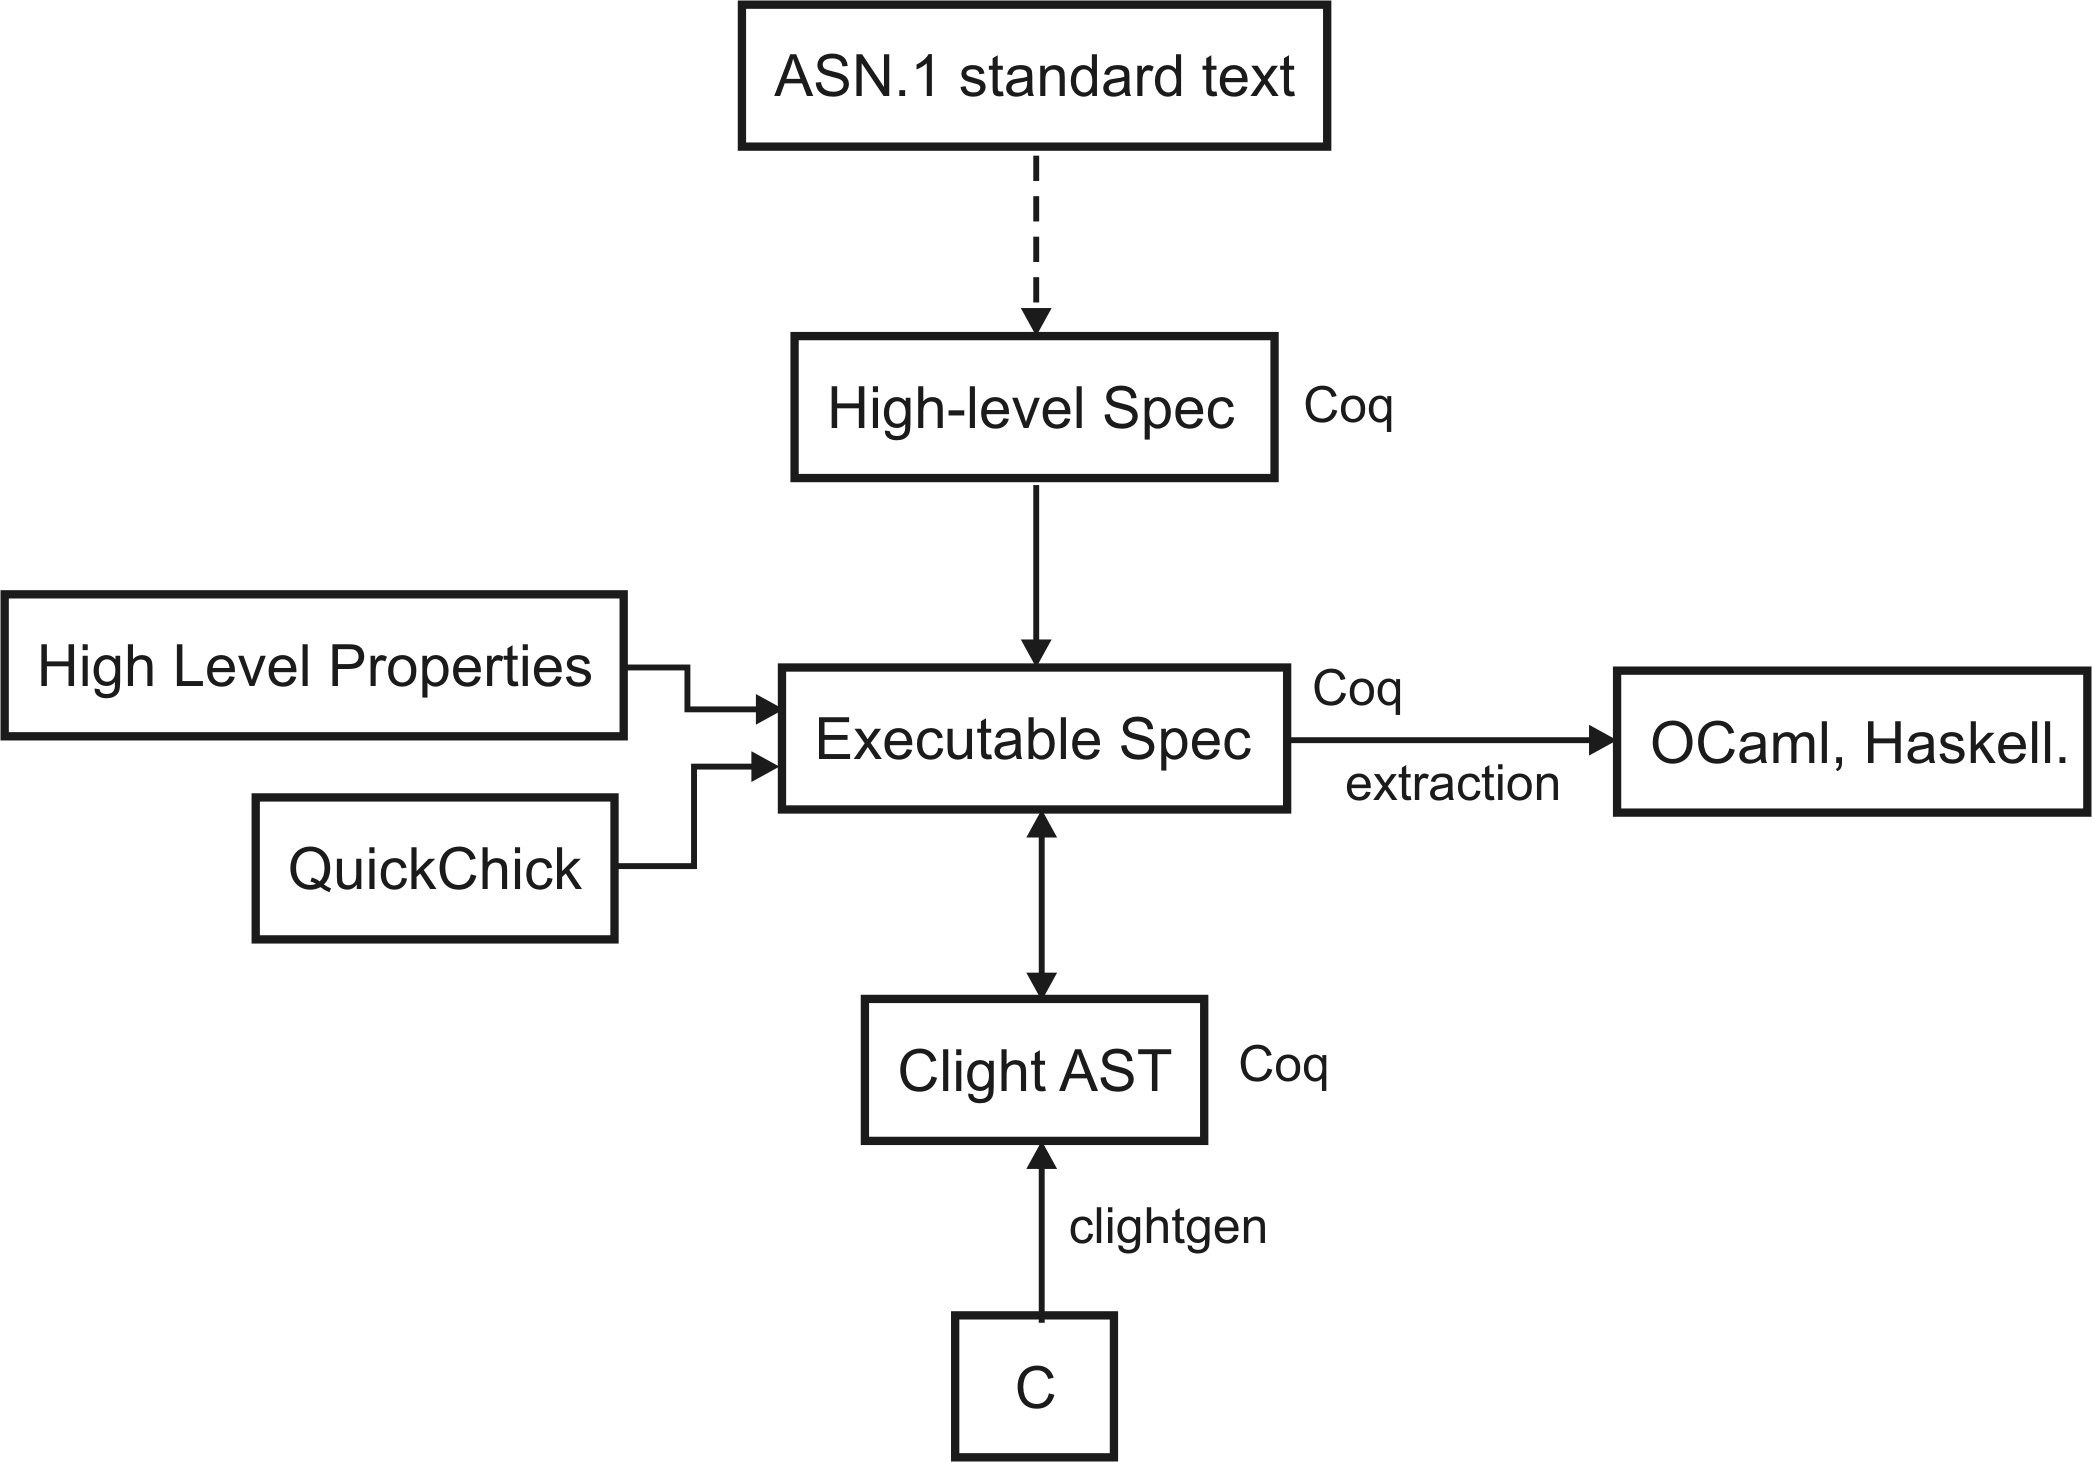
\includegraphics[width=10cm]{VerificationArchitectureDiagram.png}

The project begins with ITU-T standard document in the form of human-readable text.
We manually convert it into formal specification (H.SPEC). This is high-level specification (in Coq) which describes the correspondence between data types (such as integers) and packet octets data layout. This specification is one of the outputs of this project and has a value of its own.


Next level of detail is Executable Specification (E.SPEC). Also written in Coq it describes ``encoder'' and ``decoder'' for each type as a pair of pure functions. We will prove that the Executable specification encodes and decodes bytes in conformance to High-Level specification.

``High-Level Properties'' like termination, computation complexity and memory safely could be proven based on executable specification. They are shown as ``High Level”  box on the left. The executable spec contains enough information to ``extract” a fully functional encoder program in languages supported by Coq extraction mechanism (e.g. OCaml) [26]. Such a possibility is shown with the box on the left of Figure 1 although we do not plan to pursue it yet. This is approach others often take and it has some drawbacks. However, it should be noted that all the work we will do up to and including Executable Spec is compatible with this approach and if needed we can revisit it. For example, in case if we need to generate ASN.1 stack for special platforms where OCaml code opens some additional opportunities for parallelization, optimization or integration. One example of such platforms could be MirageOS [27]  which is the OCaml-based unikernel.

The box at the left marked QuickChick represents another possibility we might not pursue immediately. It is using randomized property-based automated testing based on on an executable specification to further verify its correctness. This work could be done using  QuickChick [28] in Coq. It is also could be used to generate a test-suite for extracted code.

At the bottom of Figure 1 is a box labeled ``C'' which represents the existing C code of ANS1C compiler. Using an automated conversion provided by the clightgen tool within the CompCert C compiler [3] we will convert this to an Abstract Syntax Tree (AST) [29] .(labeled ``C.AST'' in Figure 1) rendered in a subset of C-language called Clight [30]. More specifically, CompCert converts C ``concrete syntax'' to ``abstract'' Clight syntax. The resulting Clight program is just a reification of the original C program in Coq, retaining the overall structure and preserving the semantics; Clight is further assigned formal semantics by CompCert that can be used to further ``reason about'' (interrogate and analyze) programs within  Coq.

Finally, as the most critical (and laborious) step of the project, we will prove that semantics of the semantics of AST of Clight translation for each given function corresponds to executable specification. This will guarantee that the C program behaves exactly as the executable spec.

The formal certification of correctness will comprise the following three elements.

a) Formal specification of ASN.1 subset, which can be examined. 

b) Proofs of semantic equivalence between the C code and the specification (in Coq Proof Assistant [14]). From such proofs, Coq can generate a ``certificate''  which is a program in a formal language based on the Calculus of Inductive Constructions (``CIC'') [35]. The ``certificate'' allows 3rd party validation of proofs which have been developed in Coq. The Calculus of Inductive Constructions (``CIC'') is a small and mathematically well-defined formal language that serves as the underlying formal system of Coq. The generated certificate is automatically validated by the relatively small Coq kernel. Although a fraudulent certificate could hypothetically be created, it will not pass validation when submitted to the Coq kernel. The resulting outcome limits the trust need to trusting the small CIC formal language and the small Coq kernel. 

c) Proofs of additional high-level properties such as memory safety and termination. 

Element (b) ensures a bug-free standard-compliant implementation, and element (c) provides further guarantee that it could not be exploited in penetration or denial of service attacks.

Additionally, our (modified) version of ASN1C could be compiled with the certified CompCert compiler [3] to extend correctness guarantees through all levels down to machine code. These project results and product offerings will provide state-of-the-art high assurance suitable for mission-critical systems. Further, since formal verification will be layered atop of a widely used ASN.1 stack, it could be immediately offered to current users. This will open new markets by making it attractive to new users who require higher assurance levels than current non-verified implementations provide.

\subsection{Current work on executable specification}

A nice thing about \texttt{asn1c} compiler is its modular structure, so we can proceed with verification in a modular way and exploit this structure in the proof. For each constructed type its parser will correspond to calling its elements' parsers in a certain order. Hence, we can represent parsers as certain finite state machines that use information provided by the ASN.1 schema to parse the binary input. Alternatively, parsers could be represented using parser combinators mentioned earlier. Decoder functions produced by \texttt{asn1c} compiler use as input a representation of ASN.1 schema, which in Coq we can formalize as a tree.

 \begin{lstlisting}[language=Coq]
Inductive TYPE_descriptor :=
  DEF { tags : list Z ;
        elements : list TYPE_descriptor 
      }.
 \end{lstlisting}

Then a sequence decoder for example will traverse the tree and apply primitive decoders, we can represent it as function that uses nested recursion (as it is implemented in the asn1c code)
 
 \begin{lstlisting}[language=Coq]
 Fixpoint seq_decoder (X : TYPE_descriptor) (ls : list byte)  :=
    match ls with
    | [] =>  OK ls
    | [t] => MORE ls       
    | t :: l :: bs =>          
      if check_tag t (tags X)
        then
          match elements X with 
          | [] => primitive_decoder l bs 
          | XS => (fix elem_seq_decoder XS bs :=
                        match XS with
                        | [] => OK bs
                        | X :: XS =>
                          match seq_decoder X bs with
                            | OK r => elem_seq_decoder XS r 
                            | r => r
                          end
                        end) XS bs
          end
        else ERROR (l::bs)
        end.
 \end{lstlisting}

 or as a FSM (example) or as sequence combinator (example) constructed from the given \texttt{TYPE\_descriptor}.


\section{Future work: automation}


\subsection{Machine arithmetic}

The first bug is related to data type ranges and modulo integer
arithmetic. These sort of problems are fairly common and require
careful coding to be avoided. Formal verification enforces a strict
mathematical model of all computer arithmetic and invariably exposes
all such bugs. We use CompCert's \texttt{Integer} library that
provides theory of 8-, 16-, 32- and 64-bit integers and 32- and 64-bit
pointers. It has some basic lemmas, however, doing proofs by hand is
quite tedious, however automation can be achieved here for programs
that allow no overflow, since then one can use
\texttt{Micromega}
tactics for automatically solving comparisons on Z (if overflow is
allowed, it is an NP-complete problem and human input may be needed:
decidability of difference constraints for modular arithmetic (and
hence machine integer arithmetic) is NP-complete, by simple reduction
from 3-coloring\cite{PointerConstraintsNP}, whereas the same task for
full Z is linear in number of variables and constraints).


\subsection{Separation Logic}

The second problem was related to \textit{pointer aliasing}. These problems are not immediately obvious because C language does not allow us to enforce any memory aliasing restrictions (unlike, say Rust). In formal verification, there is a rigorous model to analyze such kind of problems called \textit{separation logic}. VST provides some automation related to this, however, it is not sufficient, but one can build custom libraries and if restricted to specific domain separation logic proofs can be fully automated. VST supports (undecidable) expressive dependently typed higher-order logic. The built-in tactics can solve simple goals, but much manual proof effort is required to transform the goals. The VST-floyd is based on databases of hints and separation logic lemmmas and tries to apply them in a smart way. We conjecture that the full force of separation logic is unnecessary in most cases and we could restrict ourselves to tractable fragments of separation logic, for which decision procedures has been already implemented within SMT solvers. The latter can be integrated into Coq proofs using SMTCoq\footnote{\url{https://smtcoq.github.io/}}.


\section{Related Work}

  Functional parsers (Narcissus)

  Extraction to C (Everparse, Galois)

  Project Everest [19] is our most direct thematic competition, and some of the high-level Project Everest documentation makes passing mention to ASN.1. The Project Everest stewards adopted a different approach based on F* [4], and the Project Everest ASN.1 work  appears at best still in far distant plans.

It is also noted that Galois did some work on ASN.1 verification in the past (circa 2012) [11]. It appears that Galois abandoned [12] the goal of full ASN.1 verification that we pursue in our project with our more pragmatic approach; Galois is now only exploring a limited subset ASN.1 verification adequate for the “vehicle-to-vehicle” (V2V) market [13], but that particular subset has limited broader applicability and the Galois effort appears encumbered by aspects of an unsuccessful  approach. It is noted that although our goal is eventually to verify all ASN.1, we decided to start with a different (X.509-related) subset of ASN.1; this subset is reasonably small, but X.509 is so widely used that our initial verified implementation of our chosen subset will have a large volume and wide range of immediate commercial applications.


\appendix
\clearpage
\section{\emph{asn\_strtoimax\_lim} source}
\label{sec:stritomax}

{\fontsize{8}{4}\selectfont  \lstinputlisting[language=C]{asn_strtoimax_lim_old.c}}


\bibliography{report}

\end{document}
